\documentclass[tikz,border=8pt]{standalone}
% Style commun des schémas : thème clair / sombre (couleurs des thèmes GitHub), fond transparent.
\usepackage[T1]{fontenc}
\usepackage{tgheros}
\renewcommand{\familydefault}{\sfdefault}
\usepackage{tikz}
\usetikzlibrary{positioning,arrows.meta,calc,fit,backgrounds}
\ifdefined\darktheme
  \definecolor{fg}{HTML}{E6EDF3}  \definecolor{muted}{HTML}{9198A1}
  \definecolor{line}{HTML}{8B949E} \definecolor{boxfill}{HTML}{151B23}
  \definecolor{boxline}{HTML}{3D444D}
  \definecolor{blue}{HTML}{4493F8} \definecolor{orange}{HTML}{DB6D28}
  \definecolor{green}{HTML}{3FB950} \definecolor{red}{HTML}{F85149}
  \definecolor{purple}{HTML}{AB7DF8}
\else
  \definecolor{fg}{HTML}{1F2328}  \definecolor{muted}{HTML}{59636E}
  \definecolor{line}{HTML}{59636E} \definecolor{boxfill}{HTML}{F6F8FA}
  \definecolor{boxline}{HTML}{D1D9E0}
  \definecolor{blue}{HTML}{0969DA} \definecolor{orange}{HTML}{BC4C00}
  \definecolor{green}{HTML}{1A7F37} \definecolor{red}{HTML}{CF222E}
  \definecolor{purple}{HTML}{8250DF}
\fi
\tikzset{
  every node/.style={text=fg, font=\small},
  block/.style={draw=boxline, fill=boxfill, rounded corners=3pt, line width=0.7pt,
                minimum height=11mm, minimum width=30mm, align=center, inner sep=5pt},
  sub/.style={font=\scriptsize, text=muted},
  wire/.style={line width=1pt, -{Stealth[length=2.6mm]}},
  biwire/.style={line width=1pt, {Stealth[length=2.6mm]}-{Stealth[length=2.6mm]}},
  lbl/.style={font=\scriptsize, text=muted, fill=none, inner sep=2pt},
}

\begin{document}
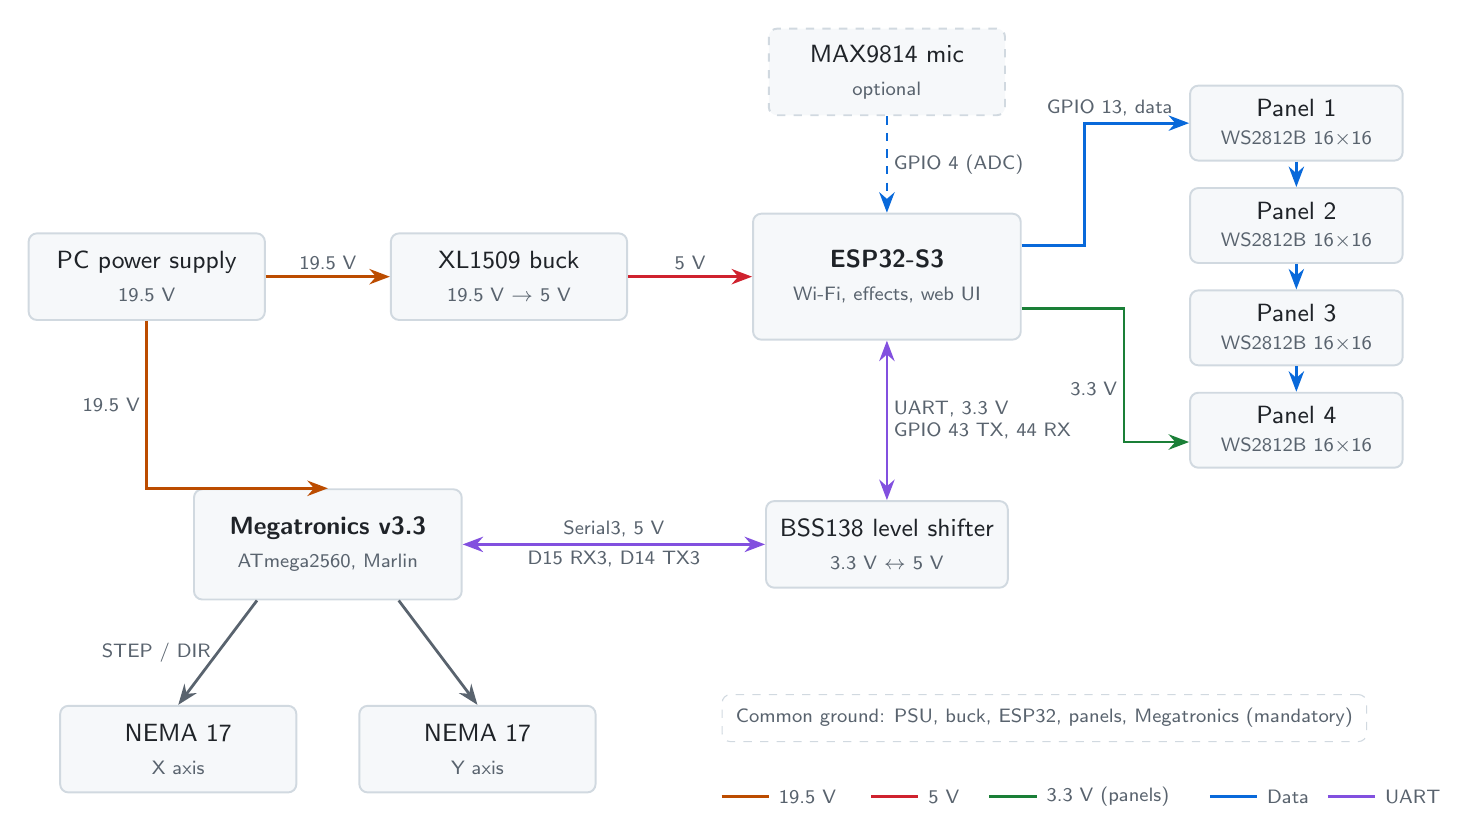
\begin{tikzpicture}[node distance=10mm]
  \node[block] (psu) at (0,0) {PC power supply\\[1pt]\textcolor{muted}{\scriptsize 19.5 V}};
  \node[block] (buck) at (4.6,0) {XL1509 buck\\[1pt]\textcolor{muted}{\scriptsize 19.5 V $\rightarrow$ 5 V}};
  \node[block, minimum width=34mm, minimum height=16mm] (esp) at (9.4,0) {\textbf{ESP32-S3}\\[1pt]\textcolor{muted}{\scriptsize Wi-Fi, effects, web UI}};
  \node[block, dashed] (mic) at (9.4,2.6) {MAX9814 mic\\[1pt]\textcolor{muted}{\scriptsize optional}};
  \foreach \i/\y in {1/1.95,2/0.65,3/-0.65,4/-1.95}
    \node[block, minimum width=27mm, minimum height=9mm] (p\i) at (14.6,\y) {Panel \i\\[-1pt]\textcolor{muted}{\scriptsize WS2812B 16$\times$16}};
  \node[block] (shift) at (9.4,-3.4) {BSS138 level shifter\\[1pt]\textcolor{muted}{\scriptsize 3.3 V $\leftrightarrow$ 5 V}};
  \node[block, minimum width=34mm, minimum height=14mm] (mega) at (2.3,-3.4) {\textbf{Megatronics v3.3}\\[1pt]\textcolor{muted}{\scriptsize ATmega2560, Marlin}};
  \node[block] (mx) at (0.4,-6.0) {NEMA 17\\[1pt]\textcolor{muted}{\scriptsize X axis}};
  \node[block] (my) at (4.2,-6.0) {NEMA 17\\[1pt]\textcolor{muted}{\scriptsize Y axis}};

  % alimentation
  \draw[wire, orange] (psu) -- node[above, lbl]{19.5 V} (buck);
  \draw[wire, orange] (psu.south) |- node[left, lbl, pos=0.25]{19.5 V} (mega.north);
  \draw[wire, red] (buck) -- node[above, lbl]{5 V} (esp);
  \draw[wire, green] ([yshift=-4mm]esp.east) -- ++(1.3,0) |- node[left, lbl, pos=0.3]{3.3 V} ([yshift=-1.5mm]p4.west);
  % données
  \draw[wire, blue] ([yshift=4mm]esp.east) -- ++(0.8,0) |- node[above, lbl, pos=0.62]{GPIO 13, data} (p1.west);
  \foreach \a/\b in {1/2,2/3,3/4} \draw[wire, blue] (p\a) -- (p\b);
  \draw[wire, blue, dashed] (mic) -- node[right, lbl]{GPIO 4 (ADC)} (esp);
  % liaison série vers les moteurs
  \draw[biwire, purple] (esp) -- node[right, lbl, align=left]{UART, 3.3 V\\GPIO 43 TX, 44 RX} (shift);
  \draw[biwire, purple] (shift) -- node[above, lbl]{Serial3, 5 V} node[below, lbl]{D15 RX3, D14 TX3} (mega);
  \draw[wire, line] (mega.south) ++(-0.9,0) -- node[left, lbl]{STEP / DIR} (mx.north);
  \draw[wire, line] (mega.south) ++(0.9,0) -- (my.north);

  % masse commune
  \node[draw=boxline, rounded corners=3pt, dashed, inner sep=5pt, font=\scriptsize, text=muted, anchor=north west]
    at (7.3,-5.3) {Common ground: PSU, buck, ESP32, panels, Megatronics (mandatory)};

  % légende
  \begin{scope}[shift={(7.3,-6.6)}]
    \foreach \c/\t/\x in {orange/19.5 V/0, red/5 V/1.9, green/3.3 V (panels)/3.4, blue/Data/6.2, purple/UART/7.7}{
      \draw[line width=1pt, \c] (\x,0) -- ++(0.6,0);
      \node[lbl, anchor=west] at (\x+0.65,0) {\t};
    }
  \end{scope}
\end{tikzpicture}
\end{document}
